\subsubsection*{BigData: A SAGA-based Pilot-Data Prototype for TROY}
\label{sec:bigdata}

\begin{figure}[t]
	\upp\upp\upp\upp
    \centering
    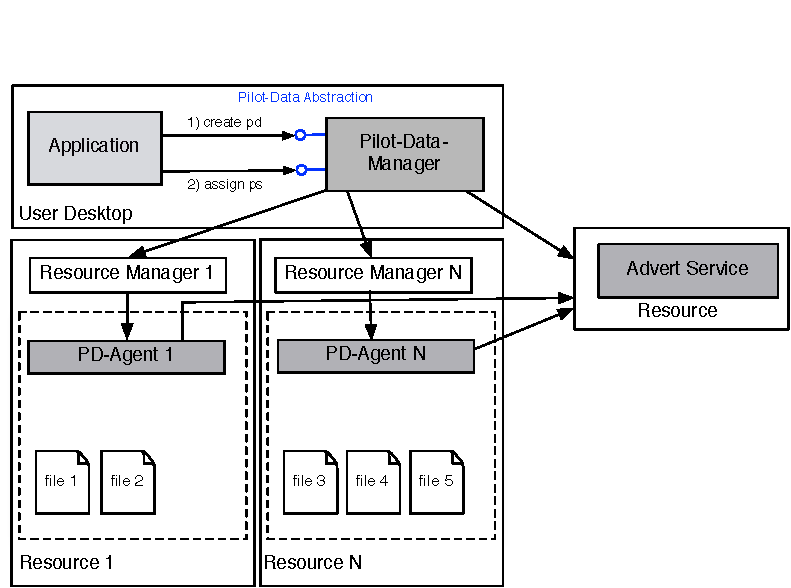
\includegraphics[width=0.48\textwidth]{figures/pilot-data-manager.pdf}
    \caption{\textbf{BigData Prototype Architecture:} The BD Manager
      exposes TROY's PD API. Application can create group of files and
      assign files to storage. The BD manager tracks file locations in
      the data catalog. The scheduler optimizes data-compute
      co-location.  The transfer manager initiates and monitors data
      movements. \up\up}
    \label{fig:pilot-data-architecture}
\end{figure}

% \begin{figure*}[t]
%   \up\up\up
%   \begin{minipage}[t]{0.475\linewidth}
%     \centering
%     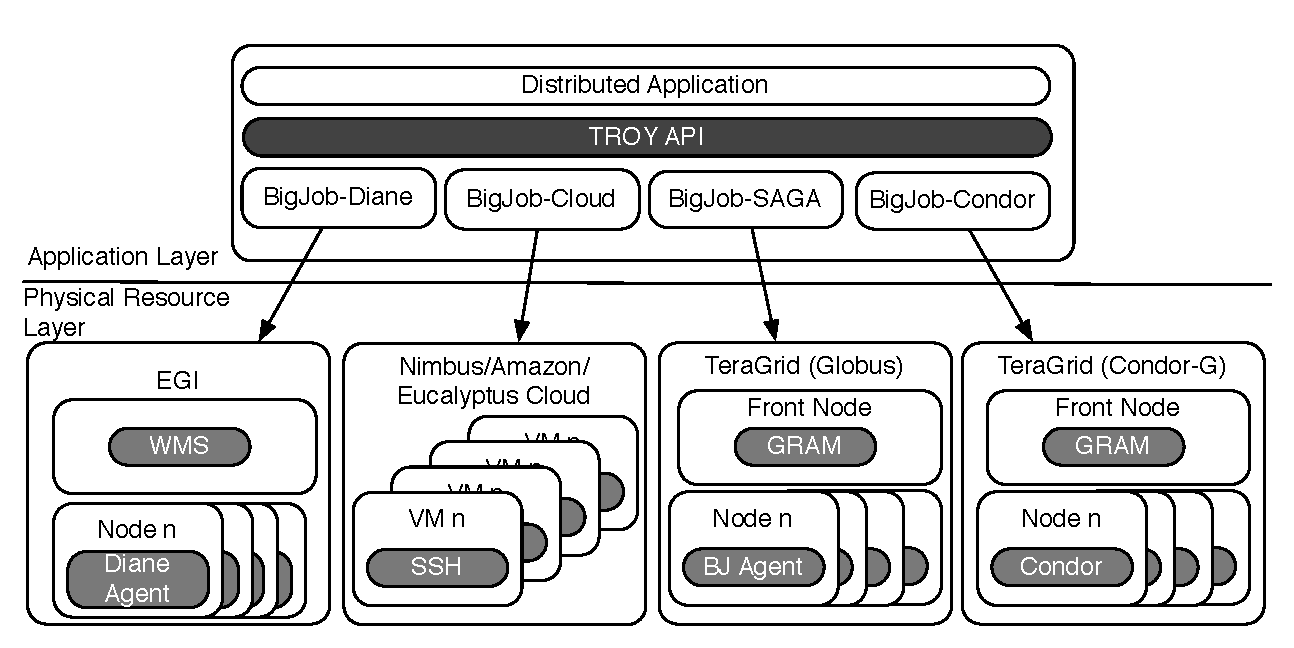
\includegraphics[width=\textwidth]{figures/distributed_pilot_job.pdf}
%     %\includegraphics[width=\textwidth]{figures/P1140340.JPG}
%     \caption{\textbf{BigJob -- SAGA-based Pilot-Job Implementation:}
%       BigJob is the implementation of the actual PJ functionality for
%       TROY. SAGA BigJob permits usage with multiple middleware
%       backends~\cite{}}
%     \label{fig:figures_distributed_pilot_job}
%     \end{minipage}
%   \hspace{0.035\linewidth}
%   \begin{minipage}[t]{0.475\linewidth}
%     \centering
%     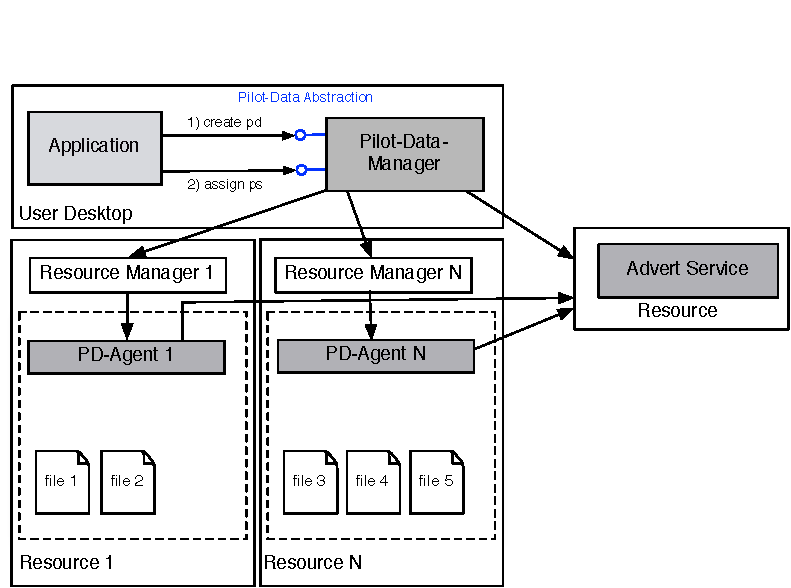
\includegraphics[width=\textwidth]{figures/pilot-data-manager.pdf}
%     \caption{\textbf{BigData Architecture:} The BD Manager exposes
%       TROY's PD API. Application can create group of files and assign 
%       files to storage. The BD manager tracks file locations in
%       the data catalog. The scheduler optimizes data-compute co-location.
%       The transfer manager initiates and monitors data movements. \up\up}
%     \label{fig:pilot-data-architecture}
%     \end{minipage}
% \end{figure*}

BigData is the SAGA-based prototype of the Pilot-Data
abstraction; in this paper it is referred to as simply
BigData (BD).  Figure~\ref{fig:pilot-data-architecture} gives an
overview of the architecture.  The system consists similarly to the BigJob 
architecture (see figure~\ref{fig:figures_re_bigjob_interactions}) of two 
components: the BD-Manager and the BD-Agents deployed on the physical
resources. The coordination scheme used is again M/W with some
intelligence that is located de-centrally at the BD-Agent. As
communication mechanism the SAGA Advert Service is used, in a similar
push/pull mode as for BJ.

The BD-Manager is responsible for (i) meta-data management, i.\,e.\ it
keeps track of the pilot stores that a pilot data object is associated
with, (ii) for scheduling data movements and data replications (taking
into account the application requirements defined via affinities), and
(iii) for managing data movements activities. For this purpose, it can rely
on external service, e.\,g.\ Globus Online for data transfer management.  
Similar to BigJob, an agent on each resource is used to manage the physical 
storage on a resource.  

A particular critical requirement for data-intensive application, is
the management of affinity between DUs and also between WUs and
DUs. The BD scheduler supports preliminary affinity-aware
scheduling: both BigJob and BigData are tightly integrated to
efficiently support compute- and data-related aspects of dynamic
execution (see also \S~\ref{sec:bigjob_description}).
 
% \jhanote{Andre, please review the next paragraph: Should it just go
%   for simplicity?} Thus, Pilot-Data introduces the PD container object
% for expressing relationships between DUs. A PD corresponds to an SU in
% the P* Model, i.\,e.\ it is used as scheduling unit for internal
% optimizations, e.\,g.\ the grouping of DUs. Having instantiated a PD,
% it can be assigned to a PS via the PD manager. A PS is a placeholder
% reserving a certain amount of storage, i.\,e.\ it corresponds to a
% pilot in the pilot-job model. By associating a PD to a PS the data is
% actually moved to the physical location associated with the PS. The PD
% manager facilitates the creation of PSs, schedules data movements
% (with respect to specified affinities) and manages data accesses.


%%%%%%%%%%%%%%%%%%%%%%%%%%%%%%%%%%%%%%%%%%%%%%%%%%%%%%%%%%%%%%%%%%%%%%


% In addition to the three Pilot-Job framework discussed in this section, various
% other frameworks exist.
% \begin{itemize}
%     \item MyCluster~\cite{1652061} enables the 
% creation of a Condor, PBS or SGE clusters on-demand.
%     \item Falkon~\cite{1362680} is a Pilot-Job framework that emphasizes the 
% performance of its task dispatcher.
%     \item Nimrod/G~\cite{10.1109/HPC.2000.846563}
%     \item DIRAC~\cite{1742-6596-219-6-062049} is another pilot-job framework 
% used by the LHCb community.
%     \item ToPoS~\cite{topos} is a REST-based web service primarily designed with 
% respect to parameter sweep applications. Internally, ToPoS utilizes PJ 
% capabilities to efficiently manage resources.
%     \item The Production and Distributed Analysis System 
% (PanDA)~\cite{1742-6596-219-6-062041} is the workload management system of 
% the ATLAS experiment. PanDA utilizes multi-user PJs for resource management. 
% The PJ component is built on top of Condor-G and referred to as AutoPilot. 
% It can also be used independently of the ATLAS environment. 
% \end{itemize}

